% Copyright (c) 2021 Tobias Briones. All rights reserved.
% SPDX-License-Identifier: CC-BY-4.0
%
% This file is part of https://github.com/tobiasbriones/
% cp-unah-mm700-agricultural-soil-sampling-for-data-analysis
%
% This source code is licensed under the Creative Commons Attribution 4.0
% International License found in the LICENSE-CC file in the root directory of
% this source tree or at https://spdx.org/licenses/CC-BY-4.0

\subsection{Proceso Propuesto}

Se va a enunciar a continuación un problema particular del proceso propuesto determinado por este estudio. El problema es un producto mínimo viable que funciona como artefacto de investigación. El problema consiste en una exageración donde se toma el cultivo de azúcares en Honduras (literalmente todo el territorio de Honduras) y el terreno se clasifica por departamento. Para obtener los estratos, como se ha mencionado previamente, es conveniente recurrir a las variedades por lo que será útil definir algunas variedades de azúcares. Por último se ha de elaborar el muestreo virtual y reporte de los datos obtenidos.

\bigbreak

El analista de datos deberá interpretar y generalizar este proceso en una base de caso por caso para poder aplicarlo correctamente. La etapa de analítica es muy pesada de trabajo ya que hay que abrir y definir junto con los demás interesados todo el contexto del problema. En este ejemplo se trata con cultivos de azúcar y un terreno ya predispuesto así como la selección de azúcares por variedad como estrategia de homogeneización. Todas estas condiciones van a cambiar en un caso real pero se pueden considerar abstraídas mediante estos resultados por lo que el analista de datos podrá ser capaz de generalizar.

\bigbreak

Los datos en particular se generarán de forma aleatoria al no contar con un conjunto de datos reales ya que esto estaría fuera del alcance de investigación.

\bigbreak

En los párrafos con un símbolo de implicación se dará una generalización del párrafo anterior para el analista de datos.

\subsubsection{Enunciado}

Asumir que en todo el territorio de Honduras se cultiva azúcar, es decir --la finca o suelo agrícola consiste en todo el territorio del país-- y se proporcionan los datos de Zafra 2021. Mediante un SIG se ha obtenido un mapa del área clasificada por departamento, en total, 18 departamentos.

\bigbreak

$\implies$ El analista de datos en esta etapa deberá contar con la muestra física y el modelo del suelo agrícola probablemente en formato shapefile (shp). Por tanto, el conjunto de datos puede comprender a cualquier tipo de  cultivo además de azúcar y cualquier zona geográfica que deberá tener
cierta delimitación geográfica.

\bigbreak

A fin de obtener los estratos se ha establecido usar la variedad --variable que define propiedades biológicas de los cultivos-- para clasificar el suelo. Al ser cosecha de azúcar, se asume que se cultivan las variedades:

\begin{itemize}
    \item Ninguna
    \item CP 72-2086
    \item Mex 69-290
    \item Mex 79-431
    \item ITV 92-1424
\end{itemize}

Las cuales son variedades muy conocidas.

\bigbreak

$\implies$ El analista obtendrá una lista mucho más grande de variedades disponibles en el suelo.

\bigbreak

Se debe de obtener un muestreo físico con la siguiente estructura mínima:

\begin{itemize}
    \item Estrato
    \item Área Cosechada (HA)
    \item TA/HA Real
\end{itemize}

Donde el conjunto de datos representa los registros tomados por el usuario en ese año de zafra.

\subsubsection{Análisis Geográfico}

Este proceso consiste en un análisis del SIG estándar. Se definen las constantes, se carga el archivo shapefile y se le da formato correspondiente agregando demás columnas. Se identifica como variable independiente a la columna departamento.

\bigbreak

El análisis del SIG da un reporte de alto nivel sobre el muestreo físico. Luego se carga el \textit{DataFrame} del muestreo físico para zafra año 2021 en este caso, entonces se desarrolla el MAS Estratificado y se establece el reporte del muestreo obtenido. Con esto, se puede hacer finalmente un análisis de fertilidad consistente y más eficiente. Por tanto, el análisis geográfico es la de las tres etapas mencionadas.

\subsubsection{Recopilación de Datos}

Este problema es una exageración que permite de momento llevar a cabo el proceso propuesto de muestreo virtual. La mayor parte de datos creados en este problema no tienen relación con la realidad pero si sirven como modelo para ser aplicado a un caso con datos reales.

\bigbreak

Los datos del muestreo físico son recolectados mediante la desnormalización de la base de datos del usuario. Esto implica que en análisis de datos se ven muchos fenómenos como redundancia, etc. El cultivo de azúcares se da por zafra, en este caso, se asume una zafra 2021 la cual da todos los registros de ese año.

\bigbreak

Las 4 \href{https://www.gob.mx/conadesuca/es/articulos/variedades-de-cana-de-azucar?idiom=es}{variedades} tomadas son una referencia importante que se encontrará de forma mucho más diversa en una base de datos real. Estas son variedades significativas, en un caso real se tiene una gran cantidad de variedades de azúcares por lo que el analista deberá tomar solo aquellas significativas para reducir la carga de la muestra. Otras variedades de azúcares significativas incluye, a saber, \textit{CP 73-1547}, \textit{RB 86-7515}, etc. Las encuestas pueden ser herramientas adecuadas para la obtención de esta información por parte de los interesados.

\bigbreak

Por tanto, se debe de tomar una variable adecuada física o biológica como la variedad del cultivo para crear cada estrato con unidades de muestreo homogéneas. Al definir inicialmente los estratos, se tendrá una lista muy grande de opciones por lo que será necesario tomar un subconjunto significativo de estos estratos filtrando aquellos que no son significativos de acuerdo al criterio establecido por el analista. Después de este filtrado, se obtienen los estratos definitivos y el mapa original queda con áreas no representativas por lo que se define el estrato vacio \textit{Ninguno}. Originalmente puede que ya existan áreas no representativas como zonas de construcción, contaminadas, etc.

\subsubsection{Filtrado}

El filtrado inicial se ha definido como sigue:

\begin{itemize}
    \item Remover estratos vacíos.
    \item Remover estratos con variedades insignificantes.
\end{itemize}

Para determinar las variedades insignificantes se establece una cota mínima (umbral) de área cosechada por variedad, estos datos vienen del muestreo físico. Por tanto, la condición para determinar si una variedad es significante es si pertenece a las cuatro variedades definidas arriba o si el área cosechada para esa variedad supera un umbral determinado. En este problema solo se filtrará tomando las cuatro variedades comúnes.

\subsubsection{Muestreo Físico}

Este \textit{DataFrame} contiene los supuestos datos de zafra $2021$ en el suelo agrícola. Es decir, todos los registros de variedades tomados en ese año. Además, en un conjunto de datos original existen muchas otras variables que pueden ser usadas para otros cálculos. Este \textit{DataFrame} solo contiene el filtrado con las columnas correspondientes para el análisis de rendimiento.

\subsubsection{Resumen de Muestro}

En las siguientes dos tablas se listan los datos del SIG y del muestreo físico filtrado para análisis de rendimiento correspondientemente.

\subsubsection{Modelo de Muestreo}

\textbf{Muestro Físico}

\bigbreak

El tamaño de la población $N = 5,000$ unidades de muestreo.

\bigbreak

Unidad de área: Hectárea.

\bigbreak

\textbf{Muestreo Virtual}

\bigbreak

\textbf{Estratos}

\bigbreak

Se han definido cuatro estratos significativos correspondientes a variedades de azúcares y uno vacío. Por tanto, $H = \{ Ninguno, H_1, ... , H_4 \}$.

\bigbreak

Tamaño de muestreo por estrato $(H_n) = t_h * factor$ donde \textit{factor} en $[0,1]$ representa el porcentaje de unidades aleatorias a tomar en cada estrato $H$ respecto a $t_h$.

\bigbreak

Con respecto al conjuntos de datos geográficos originalmente cargado, este simplemente cuenta con una (generosa) columna \textit{geography} la cual contiene la información vectorial del mapa del suelo agrícola. También fue útil la columna \textit{DEPARTMENT\_COL} conteniendo la partición hecha por el usuario. En este caso, los estratos son por variedad significante por lo que el problema debe ser tal que los subconjuntos de la partición del mapa (\say{departamentos}) contienen únicamente una variedad. Esto se detalla más en la sección de visualización abajo. A partir de estos criterios, el analista deberá poder obtener la información geográfica útil del usuario.

\subsubsection{Visualización de Muestro}

En los siguientes bloques se visualizan los datos obtenidos arriba.

\bigbreak

Por ejemplo, en los \say{departamentos} en azul (Cortés, Atlántida, Yoro,Ocotepeque, Lempira y El Paraíso) se cultiva variedad \textit{CP 72-2086}. Así, esos $6$ \say{departamentos} forman un estrato.

\subsubsection{Modelo}

El resultado del muestreo virtual se desarrolla en esta sección.

\bigbreak

Se importa el módulo de muestreo que contiene la implementación del modelo de muestreo virtual y el módulo que contiene el caso de prueba para resolución:

\bigbreak

\begin{lstlisting}[language=Python, caption=Importar dependencias]
import sampling
from test import main
\end{lstlisting}

\bigbreak

Se crea una instancia del problema conteniendo la información geográfica y muestreo físico generado con datos aleatorios. Recordar que cada vez al correr el programa se genera un problema con nuevos datos y que los datos generados aleatoriamente no producen resultados comparables a la realidad pero el proceso es totalmente válido para cualquier caso de uso tanto de prueba como real.

\bigbreak

\begin{lstlisting}[language=Python, caption=Importar dependencias]
main = main.Main.new_instance('./test')
sampling = sampling.Sampling.from_main(main)
\end{lstlisting}

\bigbreak

Imprimiendo el muestreo físico se obtuvo el conjunto de datos siguiente:

\begin{table}[H]
    \centering
    \begin{tabular}{|l|l|l|l|}
    \hline
    \rowcolor[HTML]{CBCEFB}
    \textbf{} & \textbf{Estrato} & \textbf{Área Cosechada (HA)} & \textbf{TA/HA Real} \\ \hline
    0         & CP 72-2086       & 1730.4                       & 8.6                 \\ \hline
    \rowcolor[HTML]{EFEFEF}
    1         & ITV 92-1424      & 325.6                        & 1.2                 \\ \hline
    2         & Ninguno          & 2414.6                       & 9.8                 \\ \hline
    \rowcolor[HTML]{EFEFEF}
    3         & CP 72-2086       & 3867.4                       & 9.9                 \\ \hline
    4         & Mex 69-290       & 1683.8                       & 4.2                 \\ \hline
    \end{tabular}
    \caption{Primeros datos del muestreo físico generado}
\end{table}

Donde como se estableció en el planteamiento del problema, este \textit{DataFrame} contiene $5,000$ registros.

\bigbreak

En el siguiente bloque es donde se debe configurar el modelo para que realice el muestreo:

\bigbreak

\begin{lstlisting}[language=Python, caption=Configurar el muestreo virtual]
# Configurar muestreo
sampling.stratum_sampling_size(400)

# Configurar filtr de estratos
stratum_filter = sampling.stratum_filter()
stratum_filter.area_threshold(2_480_000)

# Correr modelo de muestreo virtual
result = sampling.run()
sampled_df = result.sampling()

result.show_sampling()
result.show_stratum_filter()
\end{lstlisting}

\bigbreak

Para futuras versiones se tendrá en cuenta que se debería poder pasar el vector que define el tamaño de la muestra para cada estrato en lugar de pasar un único tamaño de la muestra para todos los estratos. Esto es, $n_h < N_h$ debería ser seleccionado para cada estrato. El resultado del muestreo da:

\begin{table}[H]
    \centering
    \begin{tabular}{|l|l|l|l|}
    \hline
    \rowcolor[HTML]{CBCEFB}
    \textbf{} & \textbf{Estrato}                                          & \textbf{Área Cosechada (HA)} & \textbf{TA/HA Real} \\ \hline
    0         & \cellcolor[HTML]{FFFFFF}{\color[HTML]{171717} CP 72-2086} & 4773.5                       & 1.4                 \\ \hline
    \rowcolor[HTML]{EFEFEF}
    1         & {\color[HTML]{171717} CP 72-2086}                         & 2341.9                       & 5.6                 \\ \hline
    2         & \cellcolor[HTML]{FFFFFF}{\color[HTML]{171717} CP 72-2086} & 148.7                        & 6.9                 \\ \hline
    \rowcolor[HTML]{EFEFEF}
    3         & {\color[HTML]{171717} CP 72-2086}                         & 1794.2                       & 0.6                 \\ \hline
    4         & \cellcolor[HTML]{FFFFFF}{\color[HTML]{171717} CP 72-2086} & 2061.7                       & 3.3                 \\ \hline
    ...       & ...                                                       & ...                          & ...                 \\ \hline
    795       & \cellcolor[HTML]{FFFFFF}{\color[HTML]{171717} Mex 79-431} & 899.8                        & 0.9                 \\ \hline
    \rowcolor[HTML]{EFEFEF}
    796       & {\color[HTML]{171717} Mex 79-431}                         & 4232.5                       & 8.9                 \\ \hline
    797       & \cellcolor[HTML]{FFFFFF}{\color[HTML]{171717} Mex 79-431} & 827.2                        & 7.5                 \\ \hline
    \rowcolor[HTML]{EFEFEF}
    798       & {\color[HTML]{171717} Mex 79-431}                         & 2025.5                       & 6.6                 \\ \hline
    799       & \cellcolor[HTML]{FFFFFF}{\color[HTML]{171717} Mex 79-431} & 4332.8                       & 4.6                 \\ \hline
    \end{tabular}
    \caption{Resultado del muestreo virtual}
\end{table}

El cual contiene $800$ registros que se comprobará que son representativos. Esto comparado a los $5,000$ registros originales. Notar que los datos se han agrupado por variedad en el resultado.

\bigbreak

Además de esto, el modelo también produce un reporte para ver el filtrado inicial que se hizo para filtrar todos aquellos estratos insignificantes. De acuerdo al valor de umbral asignado al algoritmo se obtuvieron que solo esos dos estratos son significantes:

\begin{figure}[H]
    \centering
    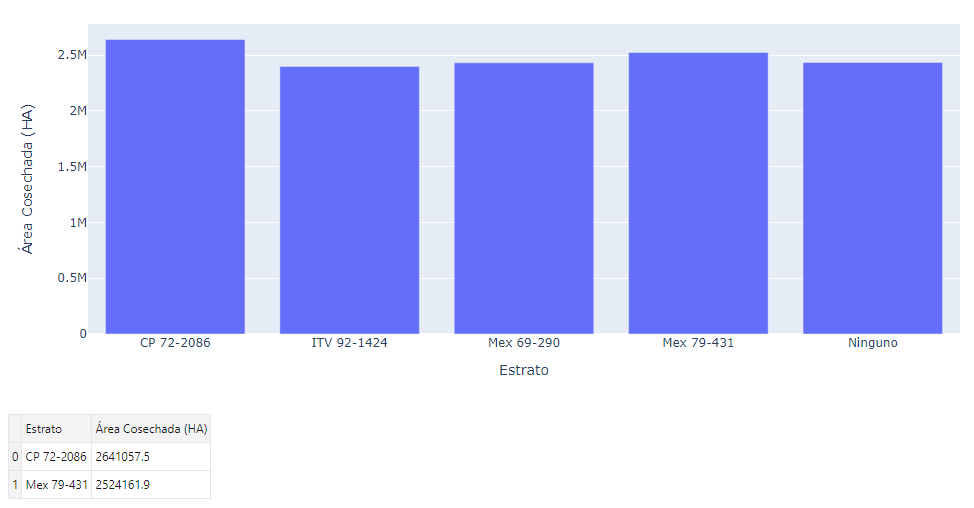
\includegraphics[width=0.3\paperwidth]{img/process-stratum-filter-report.png}
    \caption{Resultado del filtro de estratos}
\end{figure}

Por lo que las variedades (\textit{ITV 92-1424
}, $2.39938M$), (\textit{Mex 69-290}, $2.431765M$) y (\textit{Ninguno}, $2.435103M$) quedan fuera definitivamente del conjunto de datos al ser insignificantes por tener un valor de área cosechada menor al umbral establecido. Aquí también se considerará para el modelo filtrar siempre el estrato \textit{Ninguno} pero de momento, aún se toma en cuenta. En un caso real, habrán muchos más estratos y se verá que muchos son claramente insignificantes.

\bigbreak

Al tener los resultados, el analista debe poder verificar la efectividad del modelo. Esto se demuestra a continuación. Se utilizó el análisis de rendimiento como aplicación del muestro virtual.

\bigbreak

\begin{lstlisting}[language=Python, caption=Análisis de rendimiento]
# Rendimiento
def get_yield(df):
    grouped = df.groupby(hn.STRATUM_COL)
    abs_yield = grouped[hn.HardSampling.YIELD_COL].sum().reset_index()
    abs_areas = grouped[hn.HardSampling.HARVESTED_AREA_COL].sum().reset_index()
    yield_result = abs_yield.merge(abs_areas)
    yield_result["Rendimiento"] = abs_yield[hn.HardSampling.YIELD_COL] / abs_areas[hn.HardSampling.HARVESTED_AREA_COL]
    return yield_result
\end{lstlisting}

\bigbreak

Notar que se suman los valores de rendimiento y de área cosechada agrupado como estratos lo que da valores absolutos y luego se toma un valor ponderado como el rendimiento de cada variedad.

\bigbreak

Por último, se mide el error relativo al computar el rendimiento del conjunto de datos originales contra el conjunto de datos del muestro virtual:

\bigbreak

\begin{lstlisting}[language=Python, caption=Comprobación de la eficiencia del muestro virtual obtenido]
sampled_yield = get_yield(sampled_df)
real_yield = get_yield(hard_sampling)

sampled_yield['Rendimiento real'] = real_yield['Rendimiento']
sampled_yield['Error relativo (%)'] = (abs(sampled_yield['Rendimiento'] - real_yield['Rendimiento']) / real_yield['Rendimiento']) * 100
\end{lstlisting}

\bigbreak


\begin{table}[H]
    \centering
    \begin{tabular}{|l|l|l|l|l|l|l|}
    \hline
    \rowcolor[HTML]{CBCEFB}
      & Estrato    & \begin{tabular}[c]{@{}l@{}}TA/HA \\ Real\end{tabular} & \begin{tabular}[c]{@{}l@{}}Área Cosechada\\  (HA)\end{tabular} & Rendimiento & \begin{tabular}[c]{@{}l@{}}Rendimiento \\ Real\end{tabular} & \begin{tabular}[c]{@{}l@{}}Error \\ Relativo (\%)\end{tabular} \\ \hline
    0 & CP 72-2086 & 1947.6                                                & 960109.2                                                       & 0.0020285   & 0.0020283                                                   & 0.0086127                                                      \\ \hline
    \rowcolor[HTML]{EFEFEF}
    1 & Mex 79-431 & 1914.0                                                & 979276.8                                                       & 0.0019545   & 0.0020501                                                   & 4.6667605                                                      \\ \hline
    \end{tabular}
    \caption{Comparación de muestreo físico contra muestreo virtual}
\end{table}

Si el tamaño de muestra por estrato se baja a un valor demasiado pequeño el error relativo se vuelve muy grande en magnitudes de $20-150\%$ por lo cual esta es una forma de comprobar la configuración correcta del muestreo virtual.

\bigbreak

Con esta configuración el analista podrá desplegar a producción datos históricos correctamente muestreados incrementado significativamente el tiempo de ejecución de los modelos de ciencia de datos que toman como alimento estos datos históricos y que probablemente se actualizan a menudo y corren periódicamente en la nube la cual además puede tener limitaciones de recursos.
